\section{Analysis}

\subsection{Bandwidth Delay Product and Link Utilisation}
\label{sec:link}

The Bandwith-Delay Product (BDP) represents the `capacity' of a link and is calculated as:

\begin{align*}
    BDP = \text{Bandwidth (bits per second)} \times \text{Round Trip Time (seconds)}
\end{align*}

For the link between \code{pc7-082-l} and \code{pc7-085-l}, which was assumed to be 1Gbps Ethernet, the observed average RTT with RDT was 0.106ms. This yields a BDP of 13250 bytes for the link.

As RDT only sends 1312 bytes in each packet, this means that RDT achieves a link utilisation of 9.9\%.

\subsection{Maximum Theoretical Data Rate}

We can also calculate that the maximum data rate of RDT as: 

\begin{align*}
    \text{Max Data Rate} = \frac{\text{Packet Size (bits)}}{\text{RTT (seconds)}} = \frac{1312 \times 8}{0.000106} = 98.9 \text{Kbps} = 0.0989 \text{Gbps} 
\end{align*}

\subsection{Performance in Different Network Scenarios}
\label{sec:performance}

\begin{figure}[H]
\begin{center}
    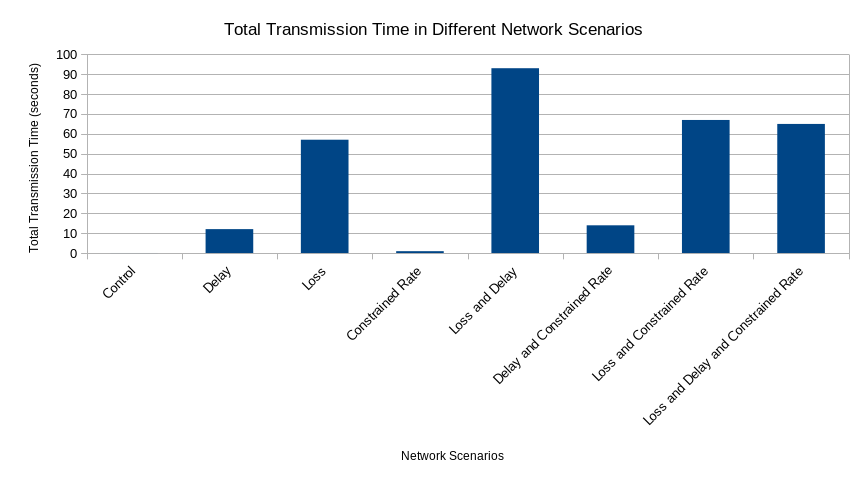
\includegraphics[width=100mm]{images/performance-network-scenarios.png}
\end{center}
\caption{Total Transmission Time in Different Network Scenarios for 230 Kb file.}\label{fig:performance}
\end{figure}

From Figure \ref{fig:performance}, we can see that the network characteristic that has the biggest impact on the performance of RDT is packet loss. Packet delay has the second greatest effect on total transmission time, with constrained data seemingly having a minimal effect. This is most likely due to the RDT data rate being less than the constrained data rate for \code{slurpe-3}.


\subsection{Efficiency of Packet Size}

We can characterise the efficiency of the RDT packet size $\rho$ as the `wastage due to control information' \cite{slides}, which for RDT is calculated as:

\begin{align*}
    \rho = \frac{i - c}{i + a} = \frac{1312 - 12}{1312 + 12} = 0.982 \text{\:(3 s.f.)}
\end{align*}